% Options for packages loaded elsewhere
\PassOptionsToPackage{unicode}{hyperref}
\PassOptionsToPackage{hyphens}{url}
%
\documentclass[
]{article}
\usepackage{amsmath,amssymb}
\usepackage{iftex}
\ifPDFTeX
  \usepackage[T1]{fontenc}
  \usepackage[utf8]{inputenc}
  \usepackage{textcomp} % provide euro and other symbols
\else % if luatex or xetex
  \usepackage{unicode-math} % this also loads fontspec
  \defaultfontfeatures{Scale=MatchLowercase}
  \defaultfontfeatures[\rmfamily]{Ligatures=TeX,Scale=1}
\fi
\usepackage{lmodern}
\ifPDFTeX\else
  % xetex/luatex font selection
\fi
% Use upquote if available, for straight quotes in verbatim environments
\IfFileExists{upquote.sty}{\usepackage{upquote}}{}
\IfFileExists{microtype.sty}{% use microtype if available
  \usepackage[]{microtype}
  \UseMicrotypeSet[protrusion]{basicmath} % disable protrusion for tt fonts
}{}
\makeatletter
\@ifundefined{KOMAClassName}{% if non-KOMA class
  \IfFileExists{parskip.sty}{%
    \usepackage{parskip}
  }{% else
    \setlength{\parindent}{0pt}
    \setlength{\parskip}{6pt plus 2pt minus 1pt}}
}{% if KOMA class
  \KOMAoptions{parskip=half}}
\makeatother
\usepackage{xcolor}
\usepackage[margin=1in]{geometry}
\usepackage{color}
\usepackage{fancyvrb}
\newcommand{\VerbBar}{|}
\newcommand{\VERB}{\Verb[commandchars=\\\{\}]}
\DefineVerbatimEnvironment{Highlighting}{Verbatim}{commandchars=\\\{\}}
% Add ',fontsize=\small' for more characters per line
\usepackage{framed}
\definecolor{shadecolor}{RGB}{248,248,248}
\newenvironment{Shaded}{\begin{snugshade}}{\end{snugshade}}
\newcommand{\AlertTok}[1]{\textcolor[rgb]{0.94,0.16,0.16}{#1}}
\newcommand{\AnnotationTok}[1]{\textcolor[rgb]{0.56,0.35,0.01}{\textbf{\textit{#1}}}}
\newcommand{\AttributeTok}[1]{\textcolor[rgb]{0.13,0.29,0.53}{#1}}
\newcommand{\BaseNTok}[1]{\textcolor[rgb]{0.00,0.00,0.81}{#1}}
\newcommand{\BuiltInTok}[1]{#1}
\newcommand{\CharTok}[1]{\textcolor[rgb]{0.31,0.60,0.02}{#1}}
\newcommand{\CommentTok}[1]{\textcolor[rgb]{0.56,0.35,0.01}{\textit{#1}}}
\newcommand{\CommentVarTok}[1]{\textcolor[rgb]{0.56,0.35,0.01}{\textbf{\textit{#1}}}}
\newcommand{\ConstantTok}[1]{\textcolor[rgb]{0.56,0.35,0.01}{#1}}
\newcommand{\ControlFlowTok}[1]{\textcolor[rgb]{0.13,0.29,0.53}{\textbf{#1}}}
\newcommand{\DataTypeTok}[1]{\textcolor[rgb]{0.13,0.29,0.53}{#1}}
\newcommand{\DecValTok}[1]{\textcolor[rgb]{0.00,0.00,0.81}{#1}}
\newcommand{\DocumentationTok}[1]{\textcolor[rgb]{0.56,0.35,0.01}{\textbf{\textit{#1}}}}
\newcommand{\ErrorTok}[1]{\textcolor[rgb]{0.64,0.00,0.00}{\textbf{#1}}}
\newcommand{\ExtensionTok}[1]{#1}
\newcommand{\FloatTok}[1]{\textcolor[rgb]{0.00,0.00,0.81}{#1}}
\newcommand{\FunctionTok}[1]{\textcolor[rgb]{0.13,0.29,0.53}{\textbf{#1}}}
\newcommand{\ImportTok}[1]{#1}
\newcommand{\InformationTok}[1]{\textcolor[rgb]{0.56,0.35,0.01}{\textbf{\textit{#1}}}}
\newcommand{\KeywordTok}[1]{\textcolor[rgb]{0.13,0.29,0.53}{\textbf{#1}}}
\newcommand{\NormalTok}[1]{#1}
\newcommand{\OperatorTok}[1]{\textcolor[rgb]{0.81,0.36,0.00}{\textbf{#1}}}
\newcommand{\OtherTok}[1]{\textcolor[rgb]{0.56,0.35,0.01}{#1}}
\newcommand{\PreprocessorTok}[1]{\textcolor[rgb]{0.56,0.35,0.01}{\textit{#1}}}
\newcommand{\RegionMarkerTok}[1]{#1}
\newcommand{\SpecialCharTok}[1]{\textcolor[rgb]{0.81,0.36,0.00}{\textbf{#1}}}
\newcommand{\SpecialStringTok}[1]{\textcolor[rgb]{0.31,0.60,0.02}{#1}}
\newcommand{\StringTok}[1]{\textcolor[rgb]{0.31,0.60,0.02}{#1}}
\newcommand{\VariableTok}[1]{\textcolor[rgb]{0.00,0.00,0.00}{#1}}
\newcommand{\VerbatimStringTok}[1]{\textcolor[rgb]{0.31,0.60,0.02}{#1}}
\newcommand{\WarningTok}[1]{\textcolor[rgb]{0.56,0.35,0.01}{\textbf{\textit{#1}}}}
\usepackage{graphicx}
\makeatletter
\def\maxwidth{\ifdim\Gin@nat@width>\linewidth\linewidth\else\Gin@nat@width\fi}
\def\maxheight{\ifdim\Gin@nat@height>\textheight\textheight\else\Gin@nat@height\fi}
\makeatother
% Scale images if necessary, so that they will not overflow the page
% margins by default, and it is still possible to overwrite the defaults
% using explicit options in \includegraphics[width, height, ...]{}
\setkeys{Gin}{width=\maxwidth,height=\maxheight,keepaspectratio}
% Set default figure placement to htbp
\makeatletter
\def\fps@figure{htbp}
\makeatother
\setlength{\emergencystretch}{3em} % prevent overfull lines
\providecommand{\tightlist}{%
  \setlength{\itemsep}{0pt}\setlength{\parskip}{0pt}}
\setcounter{secnumdepth}{-\maxdimen} % remove section numbering
\ifLuaTeX
  \usepackage{selnolig}  % disable illegal ligatures
\fi
\usepackage{bookmark}
\IfFileExists{xurl.sty}{\usepackage{xurl}}{} % add URL line breaks if available
\urlstyle{same}
\hypersetup{
  pdftitle={Resumen 1 Experimentos},
  pdfauthor={Daniel Sibaja Salazar},
  hidelinks,
  pdfcreator={LaTeX via pandoc}}

\title{Resumen 1 Experimentos}
\author{Daniel Sibaja Salazar}
\date{}

\begin{document}
\maketitle

{
\setcounter{tocdepth}{2}
\tableofcontents
}
\section{Introducción al tema}\label{introducciuxf3n-al-tema}

\subsection{Diseño de un experimento}\label{diseuxf1o-de-un-experimento}

\begin{itemize}
\item
  El experimentador hace cambio deliberados en las variables de entrada
  de un proceso o sistema. Con el fin de identificar las razones de los
  cambios que pueden observarse en la variable respuesta.
\item
  También el experimentador está interesado en el efecto de algún
  proceso o intervención, llamado tratamiento sobre la respuesta de los
  objetos u unidades experimentales.
\item
  Cuando se pueden controlar los factores se pueden llegar a
  conclusiones de causa-efecto, el cambio de tratamiento es causante del
  cambio en la respuesta.
\item
  Cuando no se pueden controlar los factores se puede llegar a
  conclusiones de correlación.
\end{itemize}

\subsubsection{Ejemplos}\label{ejemplos}

\textbf{Situación en la que el cambio de las condiciones sea la causa
del cambio en la salida:} Un experimento donde se estudia cómo
diferentes niveles de luz afectan el crecimiento de las plantas. Al
aumentar la cantidad de luz para un grupo de plantas mientras otro grupo
permanece bajo condiciones normales, se observa que las plantas con más
luz crecen significativamente más rápido. En este caso, el cambio en la
cantidad de luz es la causa del cambio en el crecimiento de las plantas.

\textbf{Situación en la que no haya certeza de que las condiciones del
factor sean la causa del cambio en la salida:} Imagina un experimento
donde se estudia el efecto de la música en el rendimiento académico de
los estudiantes. Un grupo de estudiantes escucha música mientras realiza
una prueba, mientras que otro grupo realiza la misma prueba en silencio.
Los resultados muestran que el grupo que escuchó música obtuvo mejores
resultados. Sin embargo, no podemos estar seguros de que la música sea
la causa directa de esta mejora, ya que otros factores como el estado de
ánimo de los estudiantes o la motivación podrían haber influido en los
resultados. En esta situación, aunque la salida (rendimiento académico)
está asociada con las condiciones del factor (escuchar música), no hay
certeza de que estas últimas sean la causa del cambio en la salida.

\subsection{Conceptos básicos}\label{conceptos-buxe1sicos}

\textbf{Variable respuesta:} Variable que se estudia en un experimento y
que se busca verificar si cambia al modificar las condiciones
controlables.

\textbf{Tratamiento:} Cada una de las condiciones controlables que se
modifican en un experimento.

\textbf{Factor:} Variable que se controla en un experimento y que puede
tener diferentes niveles.

\textbf{Nivel de un factor:} Cada una de las posibilidades que se
estudian de un factor.

\textbf{Efecto del tratamiento:} Diferencia entre el promedio de la
variable respuesta en un tratamiento específico y el promedio general de
la variable respuesta. Si el tratamiento no tiene efecto sobre la
respuesta el efecto es 0

\textbf{Efecto positivo del tratamiento:} El promedio de la variable
respuesta en un tratamiento específico es mayor que el promedio general.

\textbf{Efecto negativo del tratamiento:} El promedio de la variable
respuesta en un tratamiento específico es menor que el promedio general.

\textbf{Promedio general:} Promedio de la variable respuesta
considerando todos los datos de todos los tratamientos.

\section{Factores en experimentos}\label{factores-en-experimentos}

Es la varible una estudiar pero no siempre tengo control total de la
misma. Pueden ser de diseño o no de diseño.

Los no de diseño y los medibles no controlables disminuyen la
variabilidad.

Se pueden:

\begin{itemize}
\item
  Fijar: Ya no es una varible en sí. Todos los elementos son iguales.
\item
  Controlar: dependdiendo del objetivo del estudio. Como los factores de
  diseño
\item
  Libre: Puede quedar como factor de ruido.

  \begin{itemize}
  \tightlist
  \item
    Si no las puedo medir pueden meter variabilidad.
  \end{itemize}
\end{itemize}

\subsection{Elección de os niveles de un factor y
rangos.}\label{elecciuxf3n-de-os-niveles-de-un-factor-y-rangos.}

\begin{itemize}
\tightlist
\item
  Factores con pocos niveles son preferibles.
\item
  Las UE deben de ser lo más parecidas posibles.

  \begin{itemize}
  \tightlist
  \item
    Si hay diferencias en las unidades es mejor otras variables medibles
    no de diseño para menor variabilidad
  \end{itemize}
\item
  Si hay un nivel de control se refiere a que no e hace nada o se da el
  tratamiento clásico
\end{itemize}

\section{Pruebas de hipótesis.}\label{pruebas-de-hipuxf3tesis.}

\subsection{H0 o hipóteis nula.}\label{h0-o-hipuxf3teis-nula.}

\[
\mu_1=\mu_2=\mu_3=\mu_4
\]

Todos los promedios de los tratamientos son iguales

\[
\tau_1=\tau_2=\tau_3=\tau_4=0
\]

Los efectos de los tratamientos son todos iguales a 0.

\subsection{H1 o hipótesis
alternativa.}\label{h1-o-hipuxf3tesis-alternativa.}

Al menos un par de tratamientos producen medias diferentes.

El factor tiene un efecto sobre la media global.

\section{Errores}\label{errores}

\subsection{Tipo I}\label{tipo-i}

Cuando se rechaza una hippótesis siendo verdaderaa

\subsection{Tipo II}\label{tipo-ii}

Cuando no se rechaza siendo falsa

\textbf{Nota:} No conviene comparar de dos en dos las medias porque
disparo el error tipo I

\section{Error experimental}\label{error-experimental}

Las diferencias entre unidades que están bajo un mimo tratamiento se
atribuye o bien a un \emph{error experimental aleatorio} o a
\emph{factores de ruido}

El mismo es esperado incluso tomando en cuenta todos los factores que
influyen en la respuesta

\section{El modelo}\label{el-modelo}

Para la media condicional:

\[
\mu_j=\mu+\tau_j
\]

Para un observación

\[
y_{ij}=\mu+\tau_j+\epsilon_i
\]

En este caso entonces:

\begin{itemize}
\item
  El efecto de un tratamiento es lo que diferencia a la media del
  tratamiento de la media general
\item
  El error es lo que diferencia a la oservación de la media del
  tratamiento.
\end{itemize}

\subsection{Supuestos del modelo}\label{supuestos-del-modelo}

Casi los mismos de regresión

\begin{itemize}
\item
  La distribución condicional es normal. En un tratamiento específico.
\item
  Igualdad de tratamientos.
\item
  Independencia
\item
  Homocedasticidad
\end{itemize}

Entonces \(y_{ij}\) debería seguir un distriución normal con media
\(\mu_j\) y varianza \(\sigma^2\)

Y \(\epsilon_{ij}\) es normal con media 0 y varianza \(\sigma^2\)

La vaarinza no tiene subindice por la homocedasticidad.

\section{Parametrizaciones de los
modelos}\label{parametrizaciones-de-los-modelos}

Vamos a meter variables auxiliares.

\subsection{Suma nula}\label{suma-nula}

En este caso los coeficientes son 1 para el tratamiento de interés, 0
para los demás y -1 para el último.

\[
E[Y|trat_j]=\mu_j=\mu+\sum^{k-1}_{j=1}\tau_jC_j
\]

Entonces i quiero tengo interés en el segundo tratamiento tengo que

(1,0,1,0) es el vector, tomando en cuenta el intercepto

En este caso los coeficientes son los efectos.

Este es el llamado modelo grande, hay que escribir qué significan todas
las variables.

En R: options(contrasts=c(``contr.sum'',``contr.poly''))

\subsection{Tratamiento de referencia}\label{tratamiento-de-referencia}

Tengo que

\[
\mu_j=\mu_1+\sum^{k-1}_{j=2}\delta_jD_j
\] con

\[
\delta_j=\mu_j-\mu_1
\] Tomo un 1 para el tratamiento de referencia como el intercepto y para
las demás un 1 si es el de interés o un 0 si no

Por ejemplo:

\begin{itemize}
\item
  si me interesa el tratamiento 2 tengo que (1,1,0,0)
\item
  Si me interesa el tratamiento 1 tengo que (1,0,0,0)
\end{itemize}

En este caso los coeficientes son, la media del primer nivel y los demás
son la diferencia que hay entre el primer nivel y el nivel que estamos
viendo.

Este es el llamado modelo grande, hay que escribir qué significan todas
las variables.

En R: options(contrasts=c(``contr.treatment'',``contr.poly''))

\section{Análisis de varianza}\label{anuxe1lisis-de-varianza}

¿Cómo hacemos para para comprobar las hipótesis cuando queremos comparar
más de dos promedios?

Con un \emph{ANDEVA} que es una técnica estadística que nos permite
justamente eso.

En el caso más sencillo hay dos fuentes de variación

\begin{itemize}
\tightlist
\item
  \textbf{Entre} tratamientos: Cuadrado Medio de tratamientos CMTrat
\item
  \textbf{Dentro} de los tratamientos: Cuadrado medio residual CMRes
\end{itemize}

\subsection{Suma de cuadrados total}\label{suma-de-cuadrados-total}

\[SCTot=\sum^n_{i=1}(y_i-\bar y )^2\] O bien así=

\[
SCTot=SCTrat+SCRes
\]

\[
\sum^n_{i=1}( y_i-\bar y)^2
\]

\subsection{CMTrat:}\label{cmtrat}

Mide la varianción que hay entre todos los promedios de los diferentes
tratamientos.

\[
CMTrat= \frac{\sum r_j(\bar y_j-\bar y)^2}{k-1}=\frac{SCTrat}{k-1}
\]

\subsection{CMRes}\label{cmres}

Una buena estimación de la variabilidad dentro de los tratamientos es el
promedio ponderado de las varianzas de cada tratamiento.

Sirve para resumir todas la varianzas de los tratamientos en una sola
medida

\textbf{Nota:} Si el experimento no es balaceado hay que ponderar.

\[
CMRes=\frac{\sum(r_j-1)s^2_j}{n-k} = \frac{SCRes}{n-k}
\]

Si es balanceado se puede resumir a:

\[
\frac{\sum^k_{j=1}s^2_j}{k}
\]

\section{Valores esperados de los cuadrados
medios}\label{valores-esperados-de-los-cuadrados-medios}

\[
E(CMRes)=\sigma^2
\]

\[
E(CMtrat)=\sigma^2+\frac{\sum^k_{j=1}r_j\tau^2_j}{k-1}
\]

Bajo la hipótesis nula cierta:

Quiere decir que los \(\tau_j=0\) por lo tanto \(E(CMtrat)=\sigma^2\)

Entocnes para probar la hipótesis de que los efectos de los tratamientos
son nulos hay que probar que

\[
E(CMRes)=E(CMTrat)
\]

\section{Distribución de las sumas de
cuadrados}\label{distribuciuxf3n-de-las-sumas-de-cuadrados}

\begin{itemize}
\item
  Sean n observaciones \(y_i\) independientes provenientes de una misma
  disstribución normal con media \(\mu\) y varianza \(\sigma^2\)
\item
  La variable \(\sum^n_{i=1}\frac{(y_i-y)^2}{\sigma^2}\) sigue una
  distribución Chi cuadrado con n-1 grados de libertad
\item
  Por lo tanto: \(SCTrat/\sigma^2\) tiene dist chi con k-1 grados de
  libertad y \(SCRes/\sigma^2\) sigue una distribución chi con n-k
  grados de libertad
\end{itemize}

\subsection{Teorema de Cochran}\label{teorema-de-cochran}

Los términos \(SC_i/\sigma^2\) son variables chi cuadrado
independientes.

\subsection{Distribución del
cociente}\label{distribuciuxf3n-del-cociente}

El estadístico F se calcula de la siguiente forma:

\[
F=\frac{CMTrat}{CMRes}
\]

Hay que recordar que si se tienen dos variables chi cuadrado
independientes, el cociente de ellas entre sus respectivos grados de
libertad sigue una distribución F

Tomando esto en cuenta entonces:

\begin{itemize}
\tightlist
\item
  Si la hipótesis nula es verdadera es de esperarse que tanto el CMTrat
  como el CMRes tengan magnitudes similares.

  \begin{itemize}
  \tightlist
  \item
    Incluso CMTrat\textless CMRes
  \end{itemize}
\item
  Si H0 es falsa se espera que CMTrat\textgreater CMRes
\item
  Por lo tanto se puede usar el cociente de distribución F para hacer la
  prueba de hipótesis ya que si H0 es verdadera este valor debe de estar
  cerca de 1
\end{itemize}

Para calcular la probabilidad asociada: pf(f,k-1,n-k,lower.tail = F)

\section{Caso de un factor con dos
niveles}\label{caso-de-un-factor-con-dos-niveles}

Cuando se analiza un factor con solo dos niveles se puede usar la
distribución \(t\), se obtiene un resultado equivalente al del ANDEVA

Tengo que:

\[
H0: \mu_1=\mu_2
\]

\[
H0: \tau_1=0
\]

Entonces la hipótesis alternativa es de dos colas

\[
H1: \mu_1 \neq \mu_2
\]

Se debe de obtenr la estimación del efecto \(\hat \tau_1\) y su
desviación estándar y con ellos se calcula el estadístico t.

\[
t=\frac{\hat \tau_1}{ee_{\hat \tau_1}}
\]

Y con la ayuda de la distribución t se obtiene la probabilidad asociada.
Se utiliza una distribución t con n-k grados de libertad. Esta
probabilidad debe de ser igual a la que se obtiene con la distribución
F.

\section{Constrastes y comparaciones
múltiples.}\label{constrastes-y-comparaciones-muxfaltiples.}

Recordemos la hipótesis del modelo

\[\mu_1=\mu_2=\mu_3=\mu_4\]

O sea que todos los promedios (o efectos) son iguales, si rechazamos la
hipótesis nula, hay suficiente evidencia estadística para saber que por
lo menos hay un par de medias distinto \emph{¿Pero cuál?}

Tenemos varios casos según el interés que tengamos.

\subsection{Caso 1: comparar todos los pares de
medias.}\label{caso-1-comparar-todos-los-pares-de-medias.}

Supongamos que tenemos un experimento con un facotr y 4 niveles.
Entonces tenemos las siguientes hipótesis

\begin{enumerate}
\def\labelenumi{\arabic{enumi}.}
\tightlist
\item
  \(\mu_1=\mu_2\)
\item
  \(\mu_1=\mu_3\)
\item
  \(\mu_1=\mu_4\)
\item
  \(\mu_2=\mu_3\)
\item
  \(\mu_2=\mu_4\)
\item
  \(\mu_3=\mu_4\)
\end{enumerate}

En este caso tenemos dos opciones:

\begin{itemize}
\tightlist
\item
  Tukey, prueba que sirve específicamente para comparar todos los pares
  de promedios
\item
  Comparaciones múltiples con corrección para no inflar el error tipo I
\end{itemize}

En este caso no es necesario verificar indepencia debido a que se sabe
que si se hace de esta forma las hipótesis no son independientes.

\subsection{Caso 2: Solo comparar un promedio con los
demás.}\label{caso-2-solo-comparar-un-promedio-con-los-demuxe1s.}

\subsubsection{Caso 2.a}\label{caso-2.a}

En este caso tenemos hipótesis de este estilo.

\begin{enumerate}
\def\labelenumi{\arabic{enumi}.}
\item
  \(\mu_1=\frac{\mu_2+\mu_3+\mu_4}{3}\)
\item
  \(\mu_2=\frac{\mu_3+\mu_4}{2}\)
\end{enumerate}

Cada hipótesis significa que el promedio de los demás es igual a
\(\mu_1\) o \(\mu_2\)

En este caso solo se pueden usar contrastes, y hay que verificar
independencia para ver si se hace corrección o no

\subsubsection{Caso 3.a}\label{caso-3.a}

Tenemos hipótesis de este estilo:

\begin{enumerate}
\def\labelenumi{\arabic{enumi}.}
\tightlist
\item
  \(\mu_1=\mu_2\)
\item
  \(\mu_1=\mu_3\)
\item
  \(\mu_1=\mu_4\)
\end{enumerate}

O sea, solo comparamos un promedio con cada uno de los demás, en este
caso se debe de hacer una prueba de Dunnet

\section{Contrastes}\label{contrastes}

Un contraste es una combinación lineal L de los promedios de los
diferentes tratamientos con la condición de que la suma de los pesos sea
0.

En este caso las hipótesis a probar son, por ejemplo

\[
H0: L_1=0
\]

Contra

\[
H1: L_1 > 0
\]

\[
L=\sum_{j=1}^k c_j\mu_j
\] donde

\[
\sum_{j=1}^k c_j=0
\]

\begin{itemize}
\tightlist
\item
  Hay dos formas de estimarlos

  \begin{itemize}
  \tightlist
  \item
    Con los promedios
  \item
    Con los coeficientes
  \end{itemize}
\item
  Siempre es necesario definir si hace falta corrección o no.
\end{itemize}

\subsection{Estimación con los
promedios.}\label{estimaciuxf3n-con-los-promedios.}

Imaginemos que tenemos un experimento de un factor y 4 niveles, entonces
según lo visto tenemos que

\[L=c_1\mu_1+c_2\mu_2+c_3\mu_3+c_4\mu_4\]

Tenemos las hipótesis siguientes:

\begin{itemize}
\tightlist
\item
  \(H0: \mu_1=\mu_2\)
\item
  \(H0: \mu_2=\mu_3\)
\end{itemize}

En este caso nos conviene escribirlos de la siguiente forma.

\begin{itemize}
\tightlist
\item
  \(H0: \mu_1-\mu_2=0\)
\item
  \(H0: \mu_2-\mu_3=0\)
\end{itemize}

Dichos comparaciones es más fácil convertirlas en vectores

\[L_1=1\mu_1+-1\mu_2+0\mu_3+0\mu_4\]

Entonces tenemos un vector de C así (1,-1,0,0)

\[L_2=0\mu_1+1\mu_2+-1\mu_3+0\mu_4\]

Entonces tenemos un vector de C así (0,1,-1,0)

\subsubsection{Verificar independencia}\label{verificar-independencia}

Para verificar independencia de las hipótesis es necesario verificar la
\emph{ortogonalidad} de los vectores.

Para eso se calcula el producto punto de los vectores

\begin{Shaded}
\begin{Highlighting}[]
\NormalTok{v1}\OtherTok{=}\FunctionTok{c}\NormalTok{(}\DecValTok{1}\NormalTok{,}\SpecialCharTok{{-}}\DecValTok{1}\NormalTok{,}\DecValTok{0}\NormalTok{,}\DecValTok{0}\NormalTok{)}
\NormalTok{v2}\OtherTok{=}\FunctionTok{c}\NormalTok{(}\DecValTok{0}\NormalTok{,}\DecValTok{1}\NormalTok{,}\SpecialCharTok{{-}}\DecValTok{1}\NormalTok{,}\DecValTok{0}\NormalTok{)}

\NormalTok{v1}\SpecialCharTok{\%*\%}\NormalTok{v2}
\end{Highlighting}
\end{Shaded}

\begin{verbatim}
##      [,1]
## [1,]   -1
\end{verbatim}

\begin{Shaded}
\begin{Highlighting}[]
\FunctionTok{crossprod}\NormalTok{(v1,v2)}
\end{Highlighting}
\end{Shaded}

\begin{verbatim}
##      [,1]
## [1,]   -1
\end{verbatim}

Si el producto punto es

\begin{itemize}
\item
  =0 entonces hay independencia y no se hace corrección
\item
  != 0 entonces no hay independencia y se hace corrección (como en ese
  caso)
\end{itemize}

Veamos ahora el caso de de un factor con 3 niveles e hipótesis
distintas.

\begin{itemize}
\item
  \(H0: \mu_1=\frac{1}{2}(\mu_2+\mu_3)\)
\item
  \(H0: \mu_2=\mu_3\)
\end{itemize}

Asumiendo que \(L=c_1\mu_1+c_2\mu_2+c_3\mu_3\)

Tenemos entonces que:

\begin{itemize}
\tightlist
\item
  \(L_1 = \mu_1-\frac{1}{2}(\mu_2+\mu_3)\)
\item
  \(L_2 = \mu_2-\mu_3\)
\end{itemize}

Los vectores serían los siguientes.

\begin{itemize}
\tightlist
\item
  v1=(1,-1/2,1/2)
\item
  v2=(0,1,-1)
\end{itemize}

Podemos analizar la independencia

\begin{Shaded}
\begin{Highlighting}[]
\NormalTok{v1}\OtherTok{=}\FunctionTok{c}\NormalTok{(}\DecValTok{1}\NormalTok{,}\SpecialCharTok{{-}}\DecValTok{1}\SpecialCharTok{/}\DecValTok{2}\NormalTok{,}\DecValTok{1}\SpecialCharTok{/}\DecValTok{2}\NormalTok{)}
\NormalTok{v2}\OtherTok{=}\FunctionTok{c}\NormalTok{(}\DecValTok{0}\NormalTok{,}\DecValTok{1}\NormalTok{,}\SpecialCharTok{{-}}\DecValTok{1}\NormalTok{)}

\FunctionTok{crossprod}\NormalTok{(v1,v2)}
\end{Highlighting}
\end{Shaded}

\begin{verbatim}
##      [,1]
## [1,]   -1
\end{verbatim}

\subsection{Estimación de los
contrastes}\label{estimaciuxf3n-de-los-contrastes}

Hasta ahora estábamos trabajando con las medias poblacionales, sin
embargo, lo común es tener acceso únicamente a las medias muestrales,
por lo que es necesario estimarlo

\[
\hat L=\sum^k_{j=1}c_j\bar y_j 
\]

Cálculo del cual ocupamos su varianza y error estándar

La varianza de un contraste es la siguiente;

\[
\hat V [\hat L] = \sum^k_{j=1}c^2_j\hat V[\bar y _j]=\sum^k_{j=1}c^2_j\frac{CMRes}{r_j}=CMRes\sum^k_{j=1}\frac{c_j^2}{r_j}
\] Esta es la varianza pero ¿Cuál es el error estándar? ¿Para qué vamos
a hacer inteevalos de todas formas?

\subsubsection{Demotración}\label{demotraciuxf3n}

\subsection{Estimación con los
coeficientes}\label{estimaciuxf3n-con-los-coeficientes}

Sea \(\beta\) el vector de coeficientes del modelo y \(h_k\) el vector
de coeficientes del contraste \(L_k\) entonces: (PREGUNTAR)

\[\hat L_k = h_k\hat \beta\]

Y la varianza

\[
\hat V[\hat L_k]=h_k^T\hat V[\hat \beta]h_k
\]

En R: var=diag(t(h)\%\emph{\%vcov(mod2)\%}\%h)

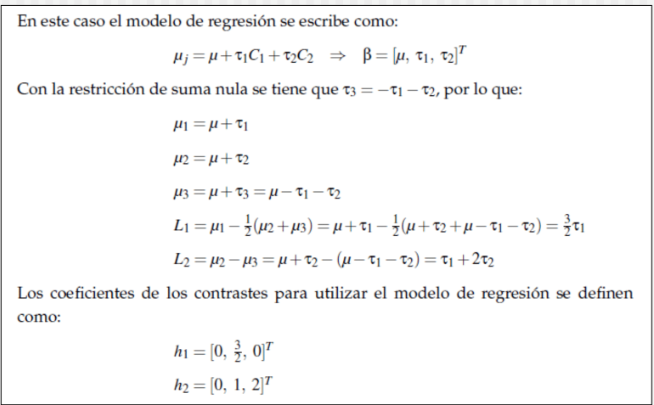
\includegraphics[width=9.08in]{../Fotos resumenes/1}

Es básicamente traducir a suma nula o tratamiento de referencia.

Antes de hacer intervalos es necesario determinar si las hipótesis
individuales se rechazan o no

Es fácil hacerlo, solo se calcula el error estándar y se estandarizan
los contrastes

\[
t=\frac{L}{ee}
\]

Y se encuentra la probabilidad asociada con \textbf{pt(t,n-k)} Si es
positivo Lower.tail=false (Es necesario verificarlo, pero mejor intentar
que L esa positivo)

\textbf{Importante:} Estas hipótesis se verifican con alfa/cantidad de
contrastes que se hacen

Para hacer intervalos de confianza se utiliza la siguiente fórmula.

\[
\hat L _k+-t_{1-\alpha/d,n-k}*\hat {ee}_k
\]

Recordar que solo se divide entre d si no hay independencia de
hipótesis.

Y la cota inferior sería

\[
\hat L _k-t_{1-\alpha/d,n-k}*\hat {ee}_k
\]

\textbf{NOTA:} es importante revisar el signo del estimador, es posible
``manipular'' las hipótesis para que siempre sean positivos.

\section{Comparaciones múltiples}\label{comparaciones-muxfaltiples}

\begin{itemize}
\item
  Para determinar cuales contrastes son diferentes de 0 se debe de
  evitar hacer pruebas simples de forma separada porque se aumenta la
  probabilidad de error tipo I
\item
  Cuando se tiene un modelo de efectos fijos, hay métodos estadísticos
  para hacer todas las comparaciones y a la vez matener el ala en un
  nivel deseado
\item
  \textbf{SI H0 NO SE RECHAZA ESTE PASO CARECE DE SENTIDO}
\end{itemize}

\subsection{Comparaciones por partes de
Tukey}\label{comparaciones-por-partes-de-tukey}

Este método toma la diferencia entre los promedios de la respuesta de
los pares posibles de los niveles de un factor.

\begin{itemize}
\item
  Evita hacer comparaciones de forma independiente
\item
  Con un número alto de tartamientos el uso de esta prueba puede
  resultar conservador, por lo cual es importante reflexionar si es
  realmente útil o no.
\item
  Cuando solo se quieren hacer contrastes para comparar los pares de
  medias, el método de Tukey produce intervalos más angostos que los de
  Bonferroni o Scheffé
\item
  Para construir un intervalo de confianza para diferencia de dos medias
  se tiene lo siguiente
\end{itemize}

\[
ee_{ij} = \sqrt{CMRes(\frac{1}{r_i}+\frac{1}{r_j})}
\]

También tenemos el estadístico

\[
q_{ij}=\frac{\bar y_i-\bar y_j}{ee_{ij}}
\]

Una vez se tiene el estadístico q para todos los pares de medias se
obtienen las probabilidades de obtener un valor igual o mayor con
\emph{la distribución de rango estundetizado de Tukey}

Y los intervalos

\[
Intervalos(1-\alpha)=(\bar y_i-\bar y_j) +- q_{\alpha,k,n-k}*ee
\]

La q tiene distribución de rango estudentizado de tukey. Estos
intervalos son solo cuando todas la diferencias son significativas

En r qtukey(1-0.05,k,n-k)

\textbf{Importante: } Estos intervalos solo se utilizan cuando es
necesario calcular todos los pares, cuando no se hace con la
distribución t.

qt(1-alfa, n-k) Es importante recordar la corrección y dividirlo entre
dos si es un intervalo.

También se puede usar el CMRes en el error estándar.

Esto tiene ventajas y desventajas:

\begin{itemize}
\item
  Al usar el CMRes se usa información de todas las varianzas, ya que el
  CMRes es una ponderación de todas las varianzas
\item
  Su uso presupone Homocedasticidad, en caso de que las varianzas no
  sean iguales, es mejor usar las varianzas de cada grupo por separado
\item
  Si se tiene el mismo tamaño de muestra iguales a ``r'' en todos los
  casos el EE se reduce
\end{itemize}

\[
EE=\sqrt{\frac{2CMRes}{r}}
\]

\begin{itemize}
\tightlist
\item
  R asume tamaños de muestra iguales y la fórmula de ``q'' ya incluye el
  2 del EE, por lo que si se calcula el EE estándar con la fórmula
  correcta (la anterior) el valor de ``q'' que se obtiene en R debe
  multiplicarse por \(\sqrt 2\) para que el resultado sea correcto.
\end{itemize}

En R: (p=ptukey(q*sqrt(2),3,97,lower.tail = F))

\section{Comparaciones por partes de
Dunnett}\label{comparaciones-por-partes-de-dunnett}

\begin{itemize}
\item
  Este método se usa solo cuando se requiere hacer comparaciones de un
  tratamiento contra todos los demás.
\item
  Estas comparaciones deben plantearse desde el diseño
\item
  Supone que es un experimento balanceado.
\end{itemize}

\section{Intervalos de confianza simultáneos y corrección de
bonferroni.}\label{intervalos-de-confianza-simultuxe1neos-y-correcciuxf3n-de-bonferroni.}

En los casos en los que se concluya que hay diferencias es importante
dar estimaciones de estas diferencias en intervalos de confianza, no
solo de forma puntual.

Es posible hacerlos de dos colas, pero en muchos experimentos se busca
maximizar o minimiar la respuesta promedio, por lo que es útil buscar
solo un límite, en este caso se busca una cota inferior para la
diferencia promedio en valor absoluto.

La cuantificación de la diferencia es muy importante para interpretar
los resultados en términos que resulten \emph{relevantes} al
investigador. La diferencia mínima representa el punto mínimo en que
teoricamente los dos promedios se deberían alejar para que resulte de
interés al investigador.

En la construcción de intervalos se debe de realizar una corrección para
asegurar una confianza global determinada.

Se recurre a la correción de \emph{bonferroni} usando el cuantil de la
distribución t con una probabilidad corregida donde:

\begin{itemize}
\item
  Si solo se hace una cota es de : \(1-\frac{\alpha}{d}\) donde d es la
  cantidad de cotas que se están construyendo.
\item
  Si se hacen intervalos es: \(1-\frac{\alpha}{2d}\) donde d es el
  número de intervalos que se están construyendo.
\end{itemize}

Se hace siempre que no haya ortogonalidad menos tukey.

\end{document}
